\documentclass{article}
\usepackage{graphicx}
\usepackage{titling}
\usepackage{listings}
\usepackage{mdframed}
\usepackage{hyperref}
\newmdenv[linecolor=black,linewidth=1.5pt]{codebox}



\title{\textbf{Software Testing Assignment 1}}
\author{\textbf{Alireza Dastmalchi Saei}\\\\
    \textit{\textbf{Student ID:} 993613026}\\\\
    \textit{\textbf{University:} University of Isfahan}\\\\
    \textit{\textbf{Course:} Software Testing Course}\\}
\date{\today}

\begin{document}

\pretitle{
  \begin{center}
  \LARGE
  
\includegraphics[width=0.4\textwidth]{pictures/university-of-isfahan-logo.png}\\[\bigskipamount]
}
\posttitle{\end{center}\vspace{3\baselineskip}}


\maketitle

\pagebreak

\section{Introduction}


In this comprehensive report, we embark on an exploration and evaluation of a Train Reservation System using a dual-approach testing methodology. Leveraging the power of JUnit and Gherkin, we conduct a thorough examination of the system's functionalities, ensuring its robustness, reliability, and adherence to business requirements.\\

JUnit, a widely adopted testing framework for Java applications, provides a solid foundation for scenario-based testing. Through the creation of five detailed scenarios, we utilize JUnit to meticulously assess various aspects of the Train Reservation System. These scenarios encompass critical functionalities such as City and Train Management, Trip Management, Ticket Booking and Cancellation, Delay Management, and Exchange Management (With Gherkin).\\

Complementing our JUnit tests, we employ Gherkin, a language-agnostic format, to write three additional scenarios. Gherkin facilitates Behavior-Driven Development (BDD) by allowing us to describe system behavior in a natural language format that is easily understandable by both technical and non-technical stakeholders.\\

This integrated approach ensures a comprehensive evaluation of the Train Reservation System, covering both the low-level unit testing provided by JUnit and the high-level behavioral testing facilitated by Gherkin. By combining these two testing methodologies, we aim to provide a robust and thorough validation of the system's functionality, ensuring its readiness for deployment in real-world scenarios.

\pagebreak

\section{Section 1: City and Train Management}
\bigskip
\bigskip
\subsection{Test Case 1.1: Add a New City}

\textbf{Description:} Verify that a new city can be added to the system.\\
\textbf{Preconditions:}
\begin{itemize}
  \item The system is running.
  \item The user is authorized to add a new city.
  \item There is new city to be added
\end{itemize}
\textbf{Steps:}
\begin{enumerate}
  \item Add a new city to the system.
\end{enumerate}
\textbf{Expected Result:} The city should be added to the list of cities in the system.

\bigskip
\hrule
\bigskip


\subsection{Test Case 1.2: Add a New Train}

\textbf{Description:} Verify that a new train can be added to the system.\\
\textbf{Preconditions:}
\begin{itemize}
  \item The system is running.
  \item The user is authorized to add a new train.
  \item There is a new train to be added.
\end{itemize}
\textbf{Steps:}
\begin{enumerate}
  \item Add a new train to the system.
\end{enumerate}
\textbf{Expected Result:} The new train should be added to the list of trains in the system.

\pagebreak

\section{Section 2: Trip Management}
\bigskip
\bigskip
\subsection{Test Case 2.1: Create a New Trip}

\textbf{Description:} Verify that a new trip can be added to the system considering the specific constraints.\\
\textbf{Preconditions:}
\begin{itemize}
  \item The system is running.
  \item The user is authorized to add a new trip.
  \item The new trip requirements are available to be created.
\end{itemize}
\textbf{Steps:}
\begin{enumerate}
  \item Provide valid details for the new trip: Origin
  \item Provide valid details for the new trip: Destination
  \item Provide valid details for the new trip: Train
  \item Provide valid details for the new trip: Departure Time
  \item Provide valid details for the new trip: Arrival Time
\end{enumerate}
\textbf{Expected Result:} The new trip should be created and registered in the system.

\bigskip
\hrule
\bigskip

\subsection{Test Case 2.2: Cancel Trip}

\textbf{Description:} Verify that a trip can be canceled in the system.\\
\textbf{Preconditions:}
\begin{itemize}
  \item The system is running.
  \item The user is authorized to cancel a trip.
\end{itemize}
\textbf{Steps:}
\begin{enumerate}
  \item Select a trip to cancel
\end{enumerate}
\textbf{Expected Result:} The selected trip should be canceled, and all associated tickets should also be canceled.

\bigskip
\hrule
\bigskip

\subsection{Test Case 2.3: Add a trip with conflicting timings to a train}

\textbf{Description:} Verify that a trip with conflicting times cannot be added to the train trips list.\\
\textbf{Preconditions:}
\begin{itemize}
  \item The system is running.
  \item The user is authorized to add a trip.
\end{itemize}
\textbf{Steps:}
\begin{enumerate}
  \item Add a valid trip to train
  \item Add a new trip that has intercepting times with previous trip
\end{enumerate}
\textbf{Expected Result:} The second should not be added to the trips list of the train, and a trip exception must be thrown.

\bigskip
\hrule
\bigskip

\subsection{Test Case 2.4: Add a trip but arrival is before departure}

\textbf{Description:} Verify that a trip with its arrival time being before departure time cannot be created\\
\textbf{Preconditions:}
\begin{itemize}
  \item The system is running.
  \item The user is authorized to add a trip.
\end{itemize}
\textbf{Steps:}
\begin{enumerate}
  \item Add an invalid trip to train (Departure time is after arrival time)
\end{enumerate}
\textbf{Expected Result:} The trip must not be created and an exception must be thrown (TripException).

\pagebreak

\section{Section 3: Ticket Booking and Cancellation}
\bigskip
\bigskip
\subsection{Test Case 3.1: Book a Ticket}

\textbf{Description:} Verify that a new ticket can be booked for a trip if the trip has not reached the maximum number of passengers.\\
\textbf{Preconditions:}
\begin{itemize}
  \item The system is running.
  \item The user is authorized to book a ticket.
  \item There is an available trip.
\end{itemize}
\textbf{Steps:}
\begin{enumerate}
  \item Select and available trip
  \item Provide passenger name
  \item Book a ticket
\end{enumerate}
\textbf{Expected Result:}  A new ticket should be booked for the selected trip.

\bigskip
\hrule
\bigskip

\subsection{Test Case 3.2: Cancel a Ticket}

\textbf{Description:} Verify that a booked ticket can be canceled.\\
\textbf{Preconditions:}
\begin{itemize}
  \item The system is running.
  \item The user has a booked ticket.
\end{itemize}
\textbf{Steps:}
\begin{enumerate}
  \item Select a booked ticket
\end{enumerate}
\textbf{Expected Result:} The selected ticket should be canceled, and the trip should be updated accordingly.

\bigskip
\hrule
\bigskip

\subsection{Test Case 3.3: Book a Ticket for a full trip}

\textbf{Description:} Verify that a ticket for a full trip cannot be created.\\
\textbf{Preconditions:}
\begin{itemize}
  \item The system is running.
\end{itemize}
\textbf{Steps:}
\begin{enumerate}
  \item Create a ticket for a trip with max passengers
\end{enumerate}
\textbf{Expected Result:} The ticket should not be booked and it must give an error.

\pagebreak

\section{Section 4: Delay Management}
\bigskip
\bigskip
\subsection{Test Case 4.1: Add Departure Delay to a Trip}

\textbf{Description:} Verify that a departure delay can be added to a trip, and it updates the real departure time.\\
\textbf{Preconditions:}
\begin{itemize}
  \item The system is running.
  \item There is a trip available for delay.
\end{itemize}
\textbf{Steps:}
\begin{enumerate}
  \item Select a trip
  \item Add departure delay
\end{enumerate}
\textbf{Expected Result:} The departure delay should be added to the trip, and the real departure time should be updated accordingly.

\bigskip
\hrule
\bigskip

\subsection{Test Case 4.2: Add Arrival Delay to a Trip}

\textbf{Description:} Verify that an arrival delay can be added to a trip, and it updates the real arrival time.\\
\textbf{Preconditions:}
\begin{itemize}
  \item The system is running.
  \item There is a trip available for delay.
\end{itemize}
\textbf{Steps:}
\begin{enumerate}
    \item Select a trip
    \item Add arrival delay
\end{enumerate}
\textbf{Expected Result:} The arrival delay should be added to the trip, and the real arrival time should be updated accordingly.

\bigskip
\hrule
\bigskip

\subsection{Test Case 4.3: Add Departure Delay More Than Duration to Pass Arrival Date}

\textbf{Description:} Verify that a departure date cannot pass arrival time after being delayed.\\
\textbf{Preconditions:}
\begin{itemize}
  \item The system is running.
  \item There is a trip available for delay.
\end{itemize}
\textbf{Steps:}
\begin{enumerate}
    \item Select a trip
    \item Add departure delay more that duration
\end{enumerate}
\textbf{Expected Result:} The departure delay should not be added to the trip, or the arrival time must be updated.

\pagebreak

\section{Section 5: Exchange Management (Cucumber)}
\bigskip
\bigskip
\subsection{Gherkin 5.1: Find All Exchangeable Tickets}

Someone wants to exchange his/her ticket, available tickets for exchanges will be shown\\
\textbf{Given} $\rightarrow$ Exchange requirements are met \\
\textbf{When} $\rightarrow$ Request to see available tickets for exchange \\
\textbf{Then} $\rightarrow$ A list of all available tickets are shown

\bigskip
\hrule
\bigskip

\subsection{Gherkin 5.2: Get previous and Next Trip of a Train}

Someone has a trip of a train and wants to see previous and next trip of that train\\
\textbf{Given} $\rightarrow$ Train has more that three trips and has a previous and next trip \\
\textbf{When} $\rightarrow$ Request to see available earlier and later trips of a train \\
\textbf{Then} $\rightarrow$ The correct successor and predecessor trips are shown

\bigskip
\hrule
\bigskip

\subsection{Gherkin 5.3: Exchange a Ticket successfully}

Someone wants to exchange his/her ticket, the exchanging process must be correct\\
\textbf{Given} $\rightarrow$ Exchanging requirements are met \\
\textbf{When} $\rightarrow$ Request to exchange a ticket from a trip \\
\textbf{Then} $\rightarrow$ Exchange must be done for a trip

\pagebreak


\section{Code Explanation and Report}
 Overall 14 test have been written (11 with JUnit and 3 with Gherkin). We will go through each one of them and explain in details if required.

 \bigskip

 \subsection{Setting Up Tests}
Setting up JUnit and Cucumber in a Maven project involves adding the necessary dependencies to the project's pom.xml file. JUnit is a widely-used testing framework for Java, while Cucumber facilitates behavior-driven development using Gherkin syntax. Below is an example passage describing how to set up these dependencies in a Maven project:\\

Must add following dependencies:
 \begin{codebox}
 \begin{lstlisting}[language=xml]
        <dependencies>
        <dependency>
            <groupId>org.junit.jupiter</groupId>
            <artifactId>junit-jupiter</artifactId>
            <version>5.8.1</version>
            <scope>test</scope>
        </dependency>

        <dependency>
            <groupId>io.cucumber</groupId>
            <artifactId>cucumber-junit</artifactId>
            <version>5.1.2</version>
            <scope>test</scope>
        </dependency>
        <dependency>
            <groupId>io.cucumber</groupId>
            <artifactId>cucumber-java</artifactId>
            <version>7.14.0</version>
            <scope>test</scope>
        </dependency>
        <dependency>
            <groupId>io.cucumber</groupId>
            <artifactId>cucumber-core</artifactId>
            <version>7.14.0</version>
        </dependency>

    </dependencies>

 \end{lstlisting}
 \end{codebox}

 \subsection{Preconditions}
In the context of JUnit testing, preconditions refer to the necessary conditions that must be satisfied before executing any test. In our case, each JUnit test requires a properly initialized instance of TicketReservationSystem to control and assess the behavior of the underlying code. \\\\\\
To enforce a consistent setup before each test, the @BeforeEach annotation is utilized in the JUnit testing framework. This annotation signifies that a designated setup method should be executed before the commencement of each individual test. In our scenario, this setup method is responsible for creating and configuring the essential instance of TicketReservationSystem.
 \bigskip

\begin{figure}[h]
  \centering
  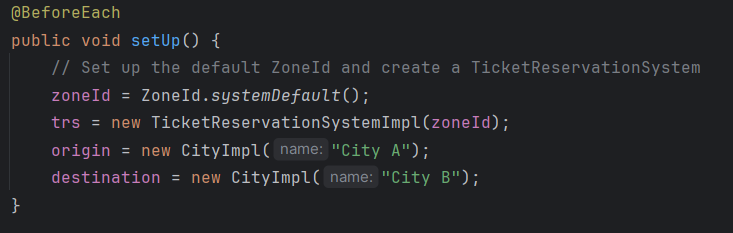
\includegraphics[width=1.0\textwidth]{pictures/T-B.png}
  \caption{Method with beforeeach}
  \label{fig:your_label}
\end{figure}

Other preconditions are not unique amongst test cases to, some preconditions are created in each test method individually. 

\pagebreak

\subsection{Section 1: City and Train Management}
\subsubsection{Test Case 1.1: Add a New City}
The code for testing if a city can be added correctly to the city list is given below:\\
First, we create a list of cities with a size of 3. Then, a new city with the name of "California" is created and added to city list. With the variable $CityExists$ and iterating through the list of all available cities, we can check if the city is in the list or not.
\begin{figure}[h]
  \centering
  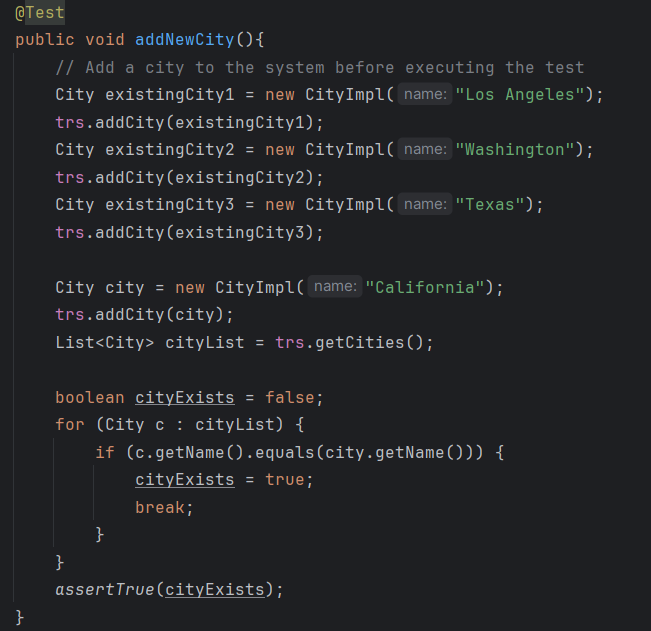
\includegraphics[width=1.0\textwidth]{pictures/T1-1.png}
  \caption{Test Case 1.1}
  \label{fig:your_label}
\end{figure}

\pagebreak

\subsubsection{Test Case 1.2: Add a New Train}
This method, checks whether a new can be added in our TrainReservationSystem correctly or not. The snippet of code can be seen below:

\begin{figure}[h]
  \centering
  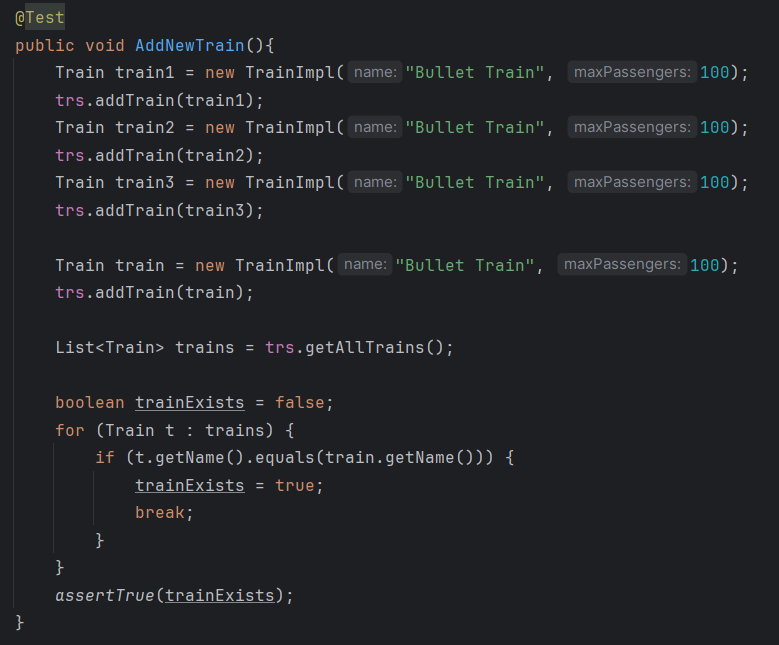
\includegraphics[width=1.0\textwidth]{pictures/T1-2.png}
  \caption{Test Case 1.2}
  \label{fig:your_label}
\end{figure}

\bigskip

As can be seen, in this test method, an initial list of 3 trains is created. Then, a new instance of train with the name of $Bullet Train$ is created and added to the list of trains. The foreach loop after adding the train, checks for the correction of process of adding new trains. The value of $trainExists$ must be true after iterating $trains$ list.

\pagebreak

\subsection{Section 2: Trip Management}
\subsubsection{Test Case 2.1: Create a New Trip}
This unittest is for testing the $createTrip$ method in the class "TrainReservationSystem". In the code, 2 trips are created and the expected list length of the trips is asserted to be 2.

\begin{figure}[h]
  \centering
  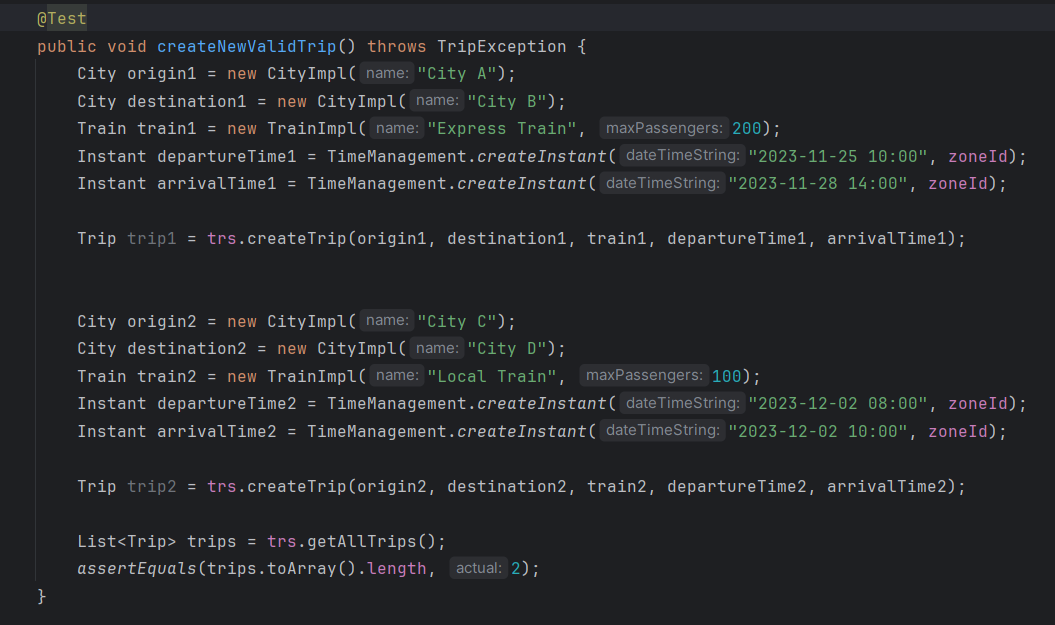
\includegraphics[width=1.0\textwidth]{pictures/T2-1.png}
  \caption{Test Case 2.1}
  \label{fig:your_label}
\end{figure}

\pagebreak

\subsubsection{Test Case 2.2: Cancel Trip}
This test case is for checking if a valid trip can be canceled correctly or not.

\begin{figure}[h]
  \centering
  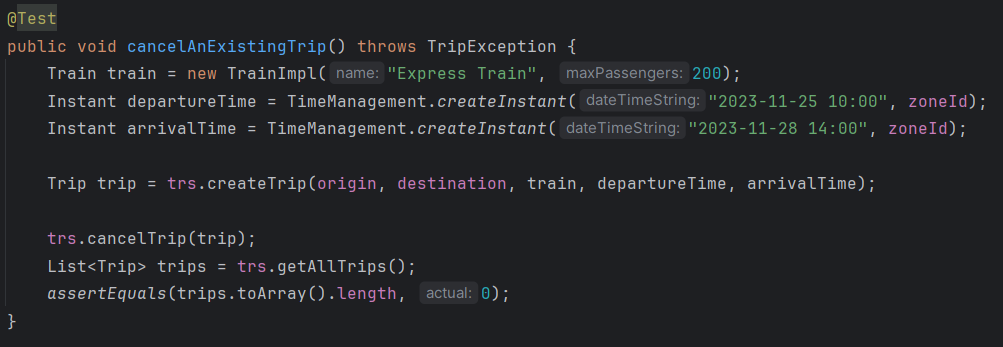
\includegraphics[width=1.0\textwidth]{pictures/T2-2.png}
  \caption{Test Case 2.2}
  \label{fig:your_label}
\end{figure}

In the code above, first we create an instance of objects needed for creating a trip, After creating the trip, we cancel the same trip created before and then check for the length of trip lists to be reduced by 1 (In this case: 0).



\subsubsection{Test Case 2.3: Add a trip with conflicting timings to a train}
In this test case, we try to create two trips for a train that they have conflicting timings and one cannot be created.

\begin{figure}[h]
  \centering
  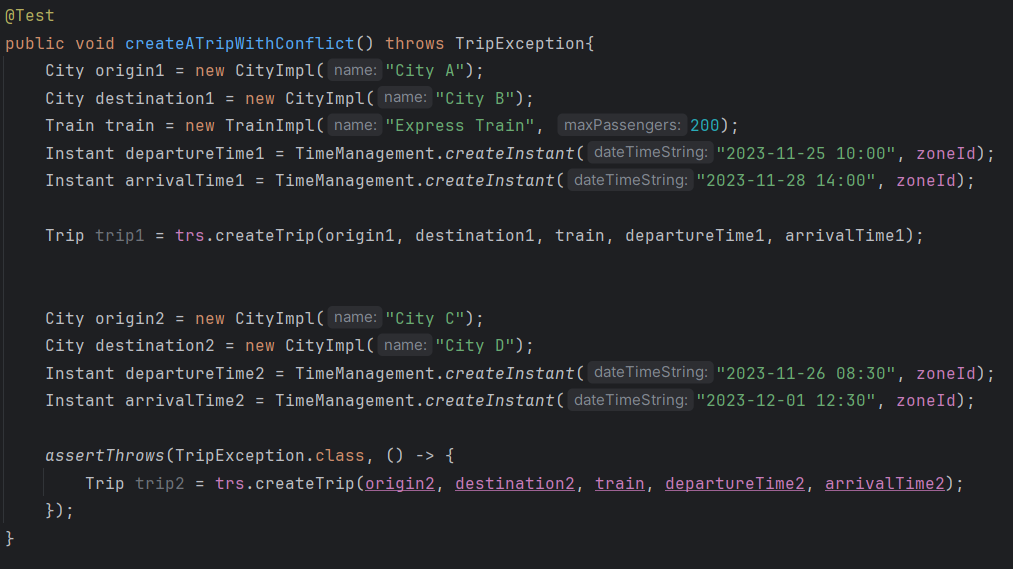
\includegraphics[width=1.0\textwidth]{pictures/T2-3.png}
  \caption{Test Case 2.3}
  \label{fig:your_label}
\end{figure}

\pagebreak

\subsubsection{Test Case 2.4: Add a trip but arrival is before departure}
In this test case we want to check if a trip can be created with its arrival time coming before departure time. This action must throw an exception. As can be seen in the picture, a trip is created and invalid timings are given to it. Then, the code expects to get a TripException.
\begin{figure}[h]
  \centering
  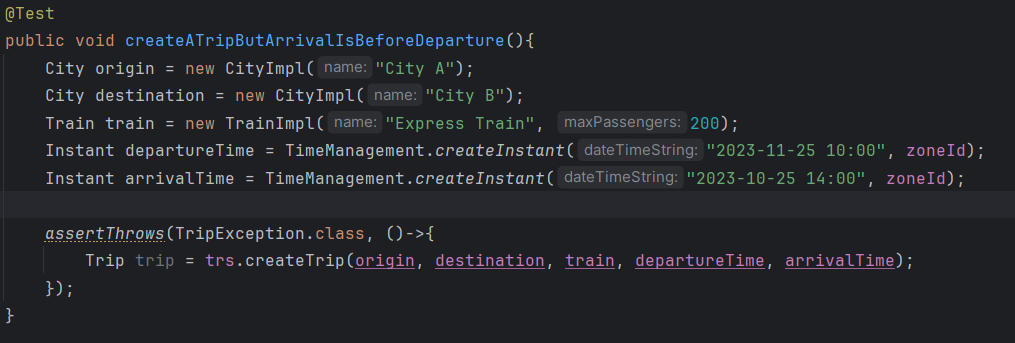
\includegraphics[width=1.0\textwidth]{pictures/T2-4.png}
  \caption{Test Case 2.4}
  \label{fig:your_label}
\end{figure}

\pagebreak

\subsection{Section 3: Ticket Booking and Cancellation}
\subsubsection{Test Case 3.1: Book a Ticket}

In this test case, we verify the system's ability to successfully book a ticket for a specified trip. The test involves creating a trip, attempting to book a ticket, and ensuring that the booked ticket is correctly registered in the system.

\begin{figure}[h]
  \centering
  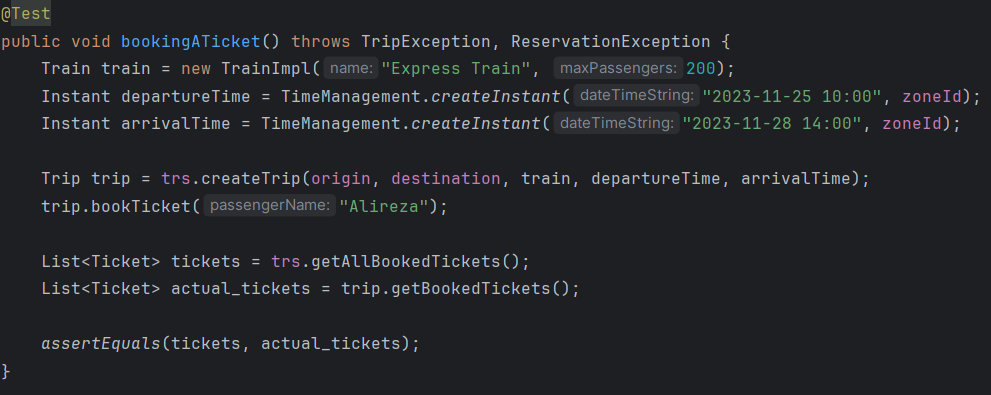
\includegraphics[width=1.0\textwidth]{pictures/T3-1.png}
  \caption{Test Case 3.1}
  \label{fig:your_label}
\end{figure}

\pagebreak

\subsubsection{Test Case 3.2: Cancel a Ticket}

This test case assesses the functionality of canceling a previously booked ticket. After booking a ticket in a given trip, the system is tested to confirm that the cancellation process correctly removes the ticket from the booked tickets list.

\begin{figure}[h]
  \centering
  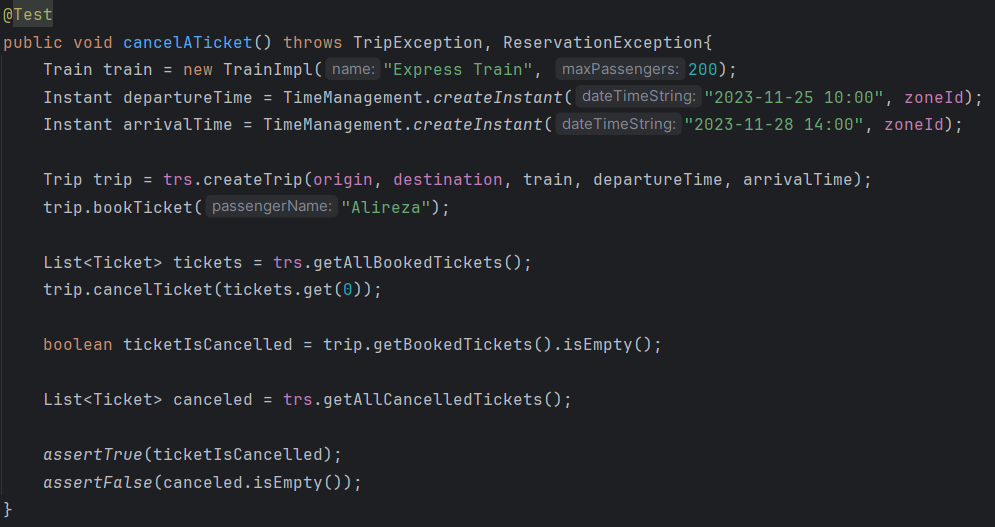
\includegraphics[width=1.0\textwidth]{pictures/T3-2.png}
  \caption{Test Case 3.2}
  \label{fig:your_label}
\end{figure}

\pagebreak

\subsubsection{Test Case 3.3: Book a Ticket for a Full Trip}

This test examines the system's behavior when attempting to book a ticket for a trip that has reached its full capacity. It checks whether the system appropriately handles scenarios where the available seats on a train are already fully booked.

\begin{figure}[h]
  \centering
  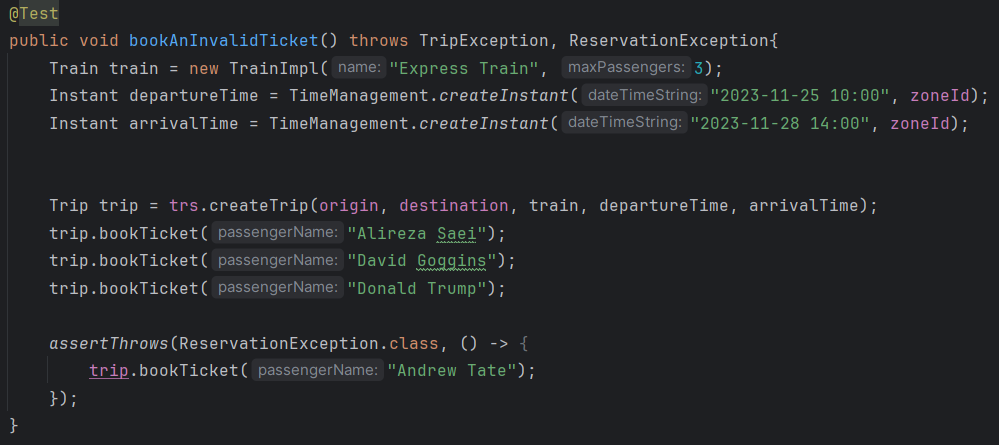
\includegraphics[width=1.0\textwidth]{pictures/T3-3.png}
  \caption{Test Case 3.3}
  \label{fig:your_label}
\end{figure}

\pagebreak

\subsection{Section 4: Delay Management}
\subsubsection{Test Case 4.1: Add Departure Delay to a Trip}

This test case verifies the system's ability to handle and correctly reflect a departure delay for a given trip. The test involves creating a trip, adding a departure delay, and checking if the system accurately records and applies the delay to the trip's schedule.

\begin{figure}[h]
  \centering
  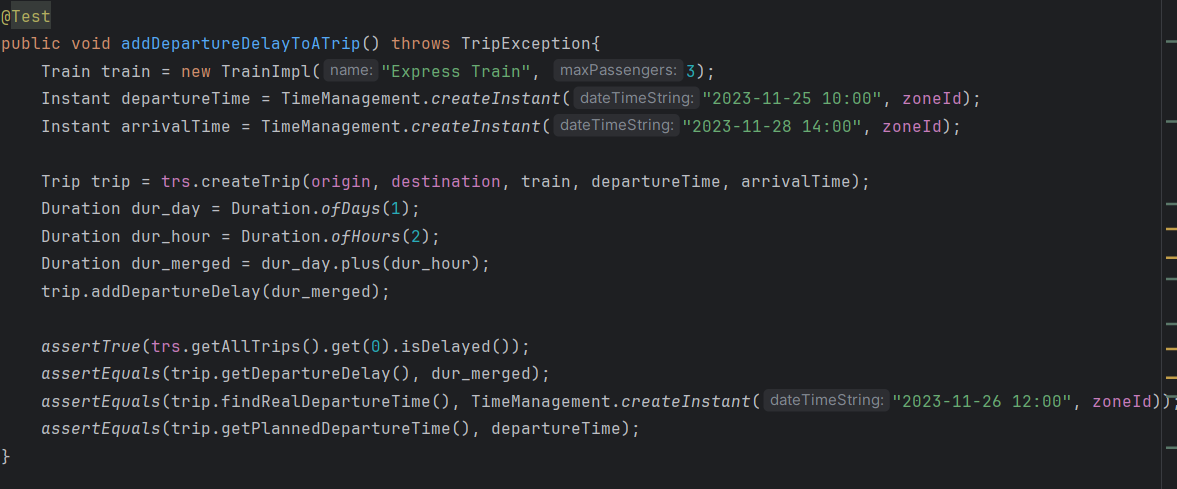
\includegraphics[width=1.0\textwidth]{pictures/T4-1.png}
  \caption{Test Case 4.1}
  \label{fig:your_label}
\end{figure}

\pagebreak

\subsubsection{Test Case 4.2: Add Arrival Delay to a Trip}

In this test case, the system's response to adding an arrival delay to a trip is evaluated. After introducing an arrival delay, the test checks whether the system appropriately updates the trip's arrival time, considering the delay.

\begin{figure}[h]
  \centering
  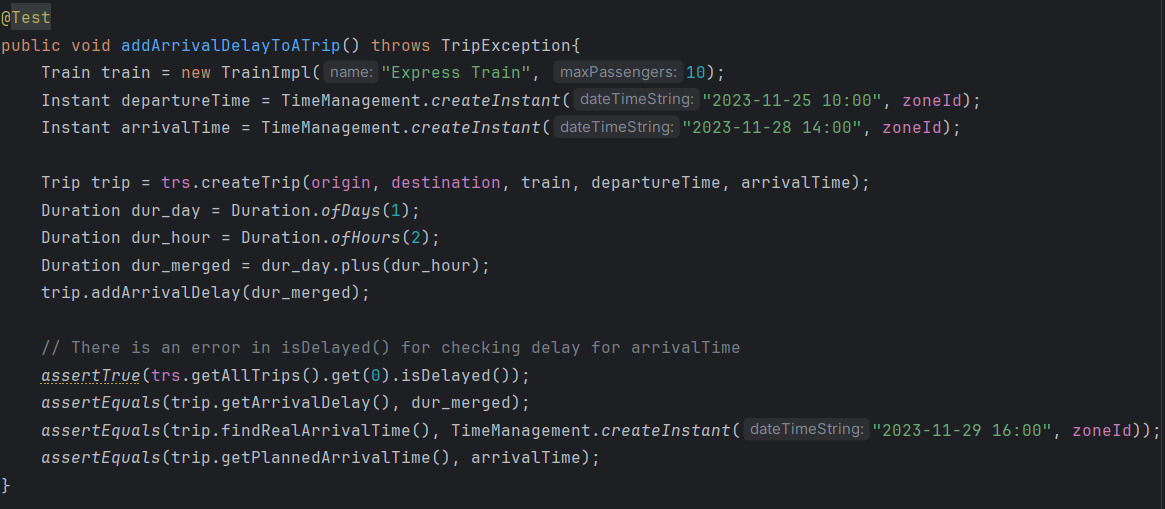
\includegraphics[width=1.0\textwidth]{pictures/T4-2.png}
  \caption{Test Case 4.2}
  \label{fig:your_label}
\end{figure}

\pagebreak

\subsubsection{Test Case 4.3: Add Departure Delay More Than Duration to Pass Arrival Date}

This test examines the system's behavior when attempting to add a departure delay that surpasses the duration needed to reach the trip's arrival date. The goal is to ensure that the system handles such cases gracefully, preventing unrealistic delays that would exceed the arrival date.

\begin{figure}[h]
  \centering
  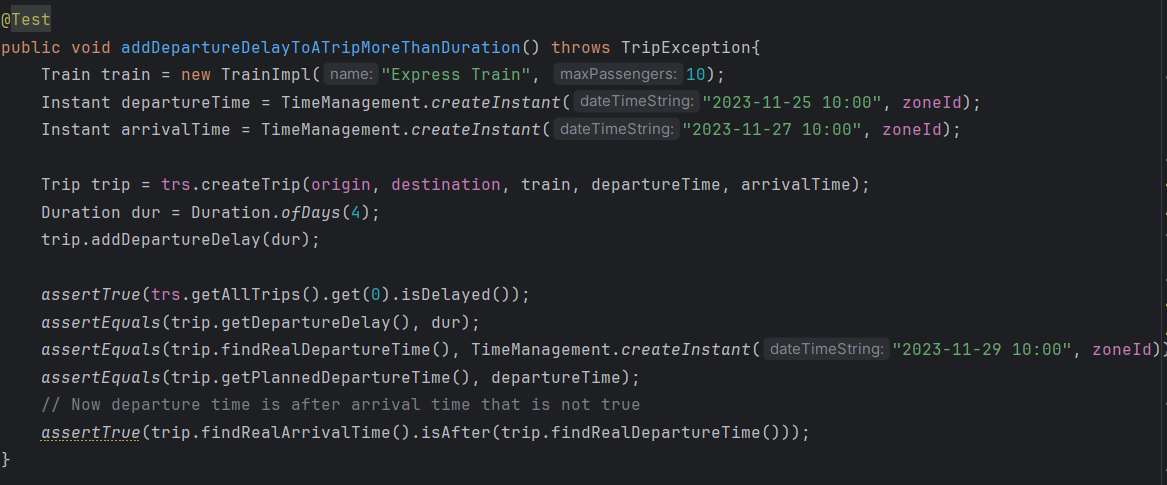
\includegraphics[width=1.0\textwidth]{pictures/T4-3.png}
  \caption{Test Case 4.2}
  \label{fig:your_label}
\end{figure}

\pagebreak

\subsection{Section 5: Exchange Management}
\subsubsection{Gherkin 5.1: Find All Exchangeable Tickets}

This Gherkin scenario outlines the steps to find all tickets that are available for exchange within the system. It likely involves identifying criteria for exchange eligibility and presenting a list of tickets that meet these criteria.

\begin{figure}[h]
  \centering
  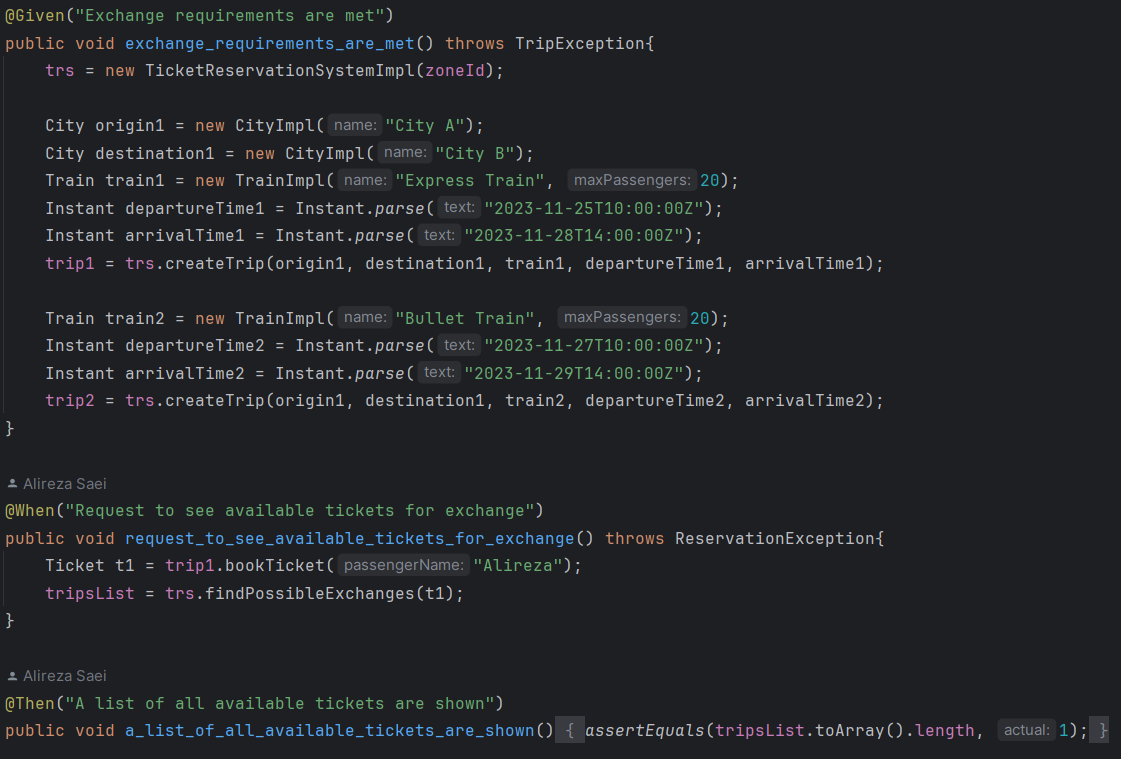
\includegraphics[width=1.0\textwidth]{pictures/T5-1.png}
  \caption{Gherkin 5.1}
  \label{fig:your_label}
\end{figure}

\pagebreak

\subsubsection{Gherkin 5.2: Get previous and Next Trip of a Train}

This Gherkin scenario focuses on retrieving information about the previous and next trips of a train. It involves interacting with the system to obtain details about the chronological order of train trips, helping users plan and manage their travel effectively.

\begin{figure}[h]
  \centering
  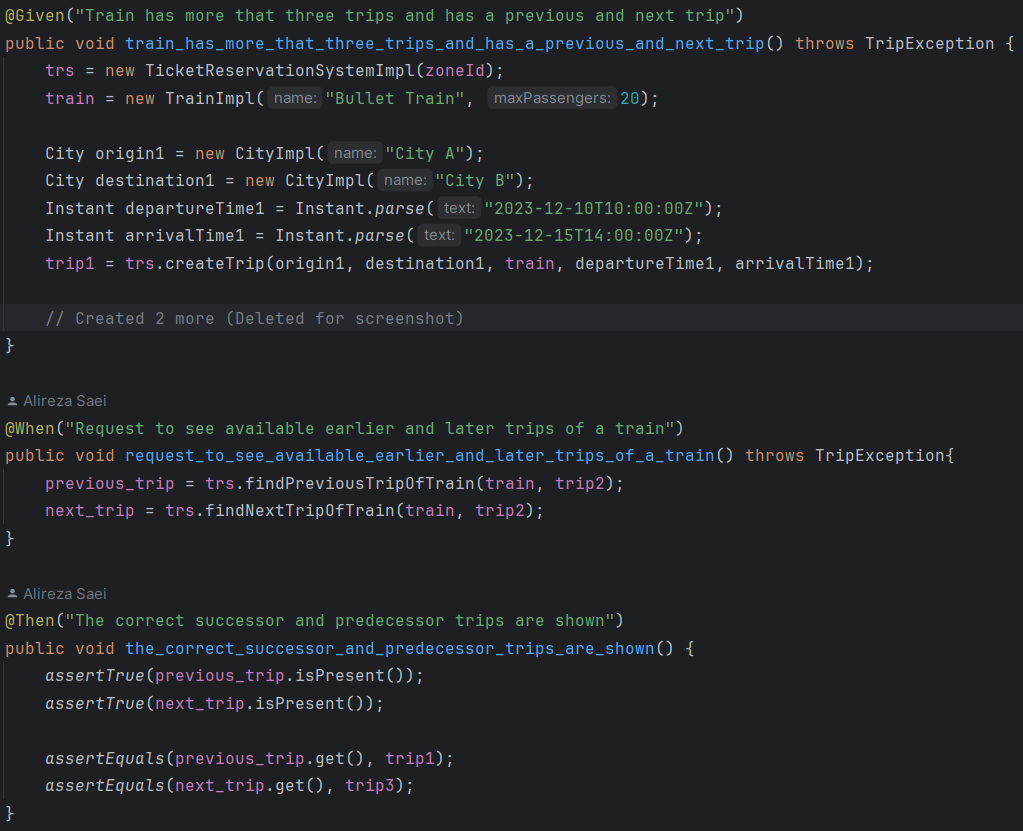
\includegraphics[width=1.0\textwidth]{pictures/T5-2.png}
  \caption{Gherkin 5.2}
  \label{fig:your_label}
\end{figure}

\pagebreak

\subsubsection{Gherkin 5.3: Exchange a Ticket successfully}

This Gherkin scenario describes the steps for successfully exchanging a ticket. It includes the process of selecting a ticket for exchange, verifying its eligibility, and executing the exchange operation, ensuring that the system handles the exchange seamlessly.

 \begin{figure}[h]
  \centering
  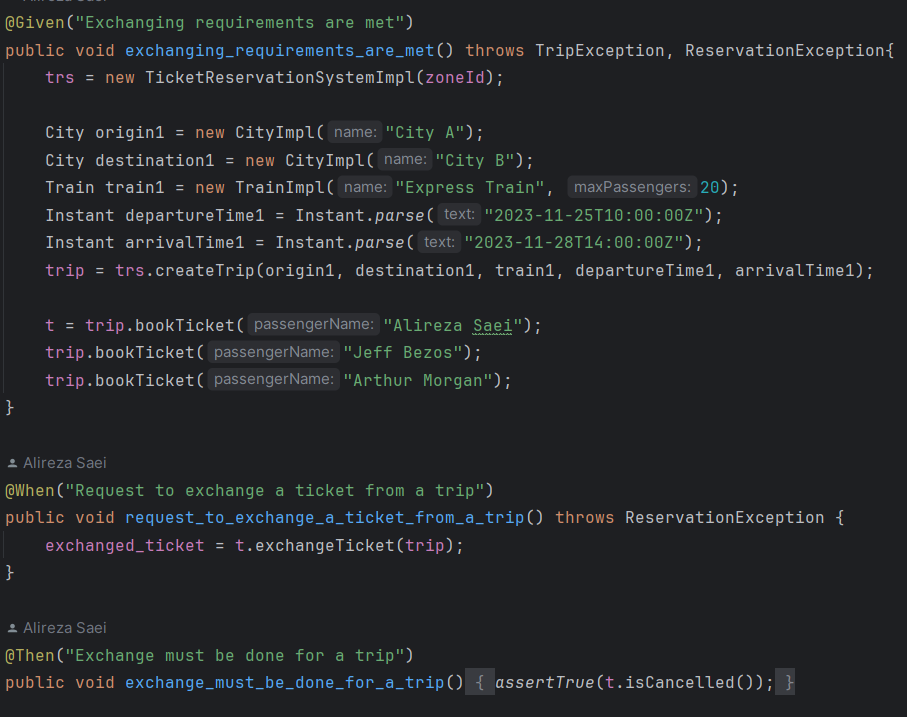
\includegraphics[width=1.0\textwidth]{pictures/T5-3.png}
  \caption{Gherkin 5.3}
  \label{fig:your_label}
\end{figure}

\pagebreak

\section{Explanation Video Link}

Click \href{https://www.example.com}{here} to see the video recorded for this Assignment.

\end{document}
